% meta.concepts: method of sections, truss
% meta.tags: realistic
% acknowledge: Peter Seiler & Luke Melander graciously shared Spring 2019 course material
% source: 2019 P. Seiler AEM2011 HW 8

Electrical transmission towers can be modeled as trusses, as shown in the figure. Although they are actually
three-dimensional space trusses, in this problem, they can be approximated as the standard two-dimensional
truss. Consider a simplified section of the transmission tower, as shown, with the following dimensions
and forces: $w = 1m$, $h = 0.5m$, $a = 0.8m$, $P = 800N$, and $Q = 1200N$. Assume that sections AC, CE, and EG
all have the same height h. You may also make use of the fact that the truss is symmetric about a vertical axis
passing through points I, J, and K. Compute the following:
\begin{enumerate}
  \item The reaction forces at supports A and B.
  \item The forces in all members enclosed by the dashed region shown in the figure.
\end{enumerate}

\begin{figure}[ht!]
  \centering
  \includegraphics[width=0.4\textwidth,
	           height=0.4\textheight,
		   keepaspectratio]{figa.png}
  \includegraphics[width=0.4\textwidth,
	           height=0.4\textheight,
		   keepaspectratio]{figb.png}
  \caption*{Electrical Transmission Tower}
\end{figure}

\iftoggle{flagSoln}{%
\vspace{.5cm}
\rule{\textwidth}{.4pt}
\vspace{.5cm}
\textbf{Solution:}
\begin{figure}[ht!]
  \centering
  \includegraphics[width=0.9\textwidth,
	           height=0.3\textheight,
		   keepaspectratio]{solna.png}
  \includegraphics[width=0.9\textwidth,
	           height=0.3\textheight,
		   keepaspectratio]{solnb.png}
  \includegraphics[width=0.9\textwidth,
	           height=0.3\textheight,
		   keepaspectratio]{solnc.png}
\end{figure}
}{%
}%
